% -----------------------------*- LaTeX -*------------------------------
\documentclass[UTF8]{report}
% ------------------------------------------------------------------------
% Packages
% ------------------------------------------------------------------------
\usepackage{ctex} % 支持中文
\usepackage[body={7in, 9in},left=1in,right=1in]{geometry} % 改变页边距
\usepackage{amsmath} % AMS 的数学宏包
\usepackage{amsfonts} % AMS 的数学字体宏包
\usepackage{amssymb} % AMS 符号库
\usepackage{bm} % 数学公式中的黑斜体
\usepackage{amsthm} % AMS 的定理环境宏包
\usepackage{graphicx} % 插图
\usepackage{subfigure} % 插子图
\usepackage{nicefrac} % 好看的分数
\usepackage{mathrsfs} % mathscr font
\usepackage{caption} % caption
\usepackage{algorithm,algorithmicx} % 伪代码支持宏包
\usepackage[noend]{algpseudocode} % 伪代码
\usepackage{fancyhdr} % 设置页眉、页脚
\usepackage{adjustbox} % 图片尺寸自动调整
\usepackage{esint} % 积分符号
\usepackage{mathtools} % 数学宏包的重要补充
\usepackage{upgreek} % 数学环境的直立希腊字母
\usepackage{enumitem} % 使用enumitem宏包, 改变列表项的格式
\usepackage{color} % 支持彩色
\usepackage{extarrows} % 任意长度的箭头
\usepackage{tikz} % 绘图
\usepackage{forest} % 绘树
\usepackage{xcolor} % 颜色宏包
\usepackage{breqn} % 公式自动换行
\usepackage{fontsize} % 字体大小
\usepackage[framemethod=TikZ]{mdframed} % 给文字加框
\usepackage{fontspec} % 字体库
\usepackage{bigstrut} % 用于表格中的换行
\usepackage{multirow} % 表格中多行单元格合并
\usepackage{multicol} % 表格中多列单元格合并
\usepackage{longtable} % 长表格
\usepackage{rotating} % 旋转图形和表格      以上三者用于绘制三线表
\usepackage{booktabs} % 三线表宏包
\usepackage{scribe} % Scribe 模板
\usepackage{diagbox} % 表格斜线
\usepackage{listings} % 插入代码
\usepackage{verbatim} % 多行注释
\usepackage{ifplatform} % 检测编译平台
\usepackage{pifont} % 圆圈数字
\usetikzlibrary{shapes.geometric, arrows} % 引入流程图需要的库
\usetikzlibrary{automata} % 引入automata库
\usetikzlibrary{shapes,arrows,positioning,chains} % 引入positioning库
% ------------------------------------------------------------------------
% Macros
% ------------------------------------------------------------------------
%~~~~~~~~~~~~~~~
% Utility latin
%~~~~~~~~~~~~~~~
\newcommand{\ie}{\textit{i.e.}}
\newcommand{\eg}{\textit{e.g.}}
%~~~~~~~~~~~~~~~
% Environment shortcuts
%~~~~~~~~~~~~~~~
\newcommand{\balign}[1]{\ealign{\begin{align}#1\end{align}}}
\newcommand{\baligns}[1]{\ealigns{\begin{align*}#1\end{align*}}}
\newcommand{\bitemize}[1]{\eitemize{\begin{itemize}#1\end{itemize}}}
\newcommand{\benumerate}[1]{\eenumerate{\begin{enumerate}#1\end{enumerate}}}
%~~~~~~~~~~~~~~~
% Text with quads around it
%~~~~~~~~~~~~~~~
\newcommand{\qtext}[1]{\quad\text{#1}\quad}
%~~~~~~~~~~~~~~~
% Shorthand for math formatting
%~~~~~~~~~~~~~~~
\newcommand{\mbb}[1]{\mathbb{#1}}
\newcommand{\mbi}[1]{\boldsymbol{#1}} % Bold and italic (math bold italic)
\newcommand{\mbf}[1]{\mathbf{#1}}
\newcommand{\mc}[1]{\mathcal{#1}}
\newcommand{\mrm}[1]{\mathrm{#1}}
\newcommand{\tbf}[1]{\textbf{#1}}
\newcommand{\tsc}[1]{\textsc{#1}}
%\def\\langle {{\langle }}
%\def\\rangle {{\rangle }}
\newcommand{\sT}{\sf T}
\newcommand{\grad}{\nabla}
\newcommand{\Proj}{\Pi}
%~~~~~~~~~~~~~~~
% Common sets 定义数集符号
%~~~~~~~~~~~~~~~
\newcommand{\R}{\mathbb{R}}
\newcommand{\Z}{\mathbb{Z}}
\newcommand{\Q}{\mathbb{Q}}
\newcommand{\N}{\mathbb{N}}
\newcommand{\C}{\mathbb{C}}
\newcommand{\reals}{\mathbb{R}} % Real number symbol
\newcommand{\integers}{\mathbb{Z}} % Integer symbol
\newcommand{\rationals}{\mathbb{Q}} % Rational numbers
\newcommand{\naturals}{\mathbb{N}} % Natural numbers
\newcommand{\complex}{\mathbb{C}} % Complex numbers
%~~~~~~~~~~~~~~~
% Common functions
%~~~~~~~~~~~~~~~
\renewcommand{\exp}[1]{\operatorname{exp}\left(#1\right)} % Exponential
\newcommand{\indic}[1]{\mbb{I}\left(#1\right)} % Indicator function
\newcommand{\indicsub}[2]{\mbb{I}_{#2}\left(#1\right)} % Indicator function
\newcommand{\argmax}{\mathop\mathrm{arg\, max}} % Defining math symbols
\newcommand{\argmin}{\mathop\mathrm{arg\, min}}
\renewcommand{\arccos}{\mathop\mathrm{arccos}}
\newcommand{\dom}{\mathop\mathrm{dom}} % Domain
\newcommand{\range}{\mathop\mathrm{range}} % Range
\newcommand{\diag}{\mathop\mathrm{diag}}
\newcommand{\tr}{\mathop\mathrm{tr}}
\newcommand{\abs}{\mathop\mathrm{abs}}
\newcommand{\card}{\mathop\mathrm{card}}
\newcommand{\sign}{\mathop\mathrm{sign}}
\newcommand{\prox}{\mathrm{prox}} % prox
\newcommand{\rank}[1]{\mathrm{rank}(#1)}
\newcommand{\supp}[1]{\mathrm{supp}(#1)}
\newcommand{\norm}[1]{\lVert#1\rVert}
%~~~~~~~~~~~~~~~
% Common probability symbols
%~~~~~~~~~~~~~~~
\newcommand{\family}{\mathcal{P}} % probability family / statistical model
\newcommand{\iid}{\stackrel{\mathrm{iid}}{\sim}}
\newcommand{\ind}{\stackrel{\mathrm{ind}}{\sim}}
\newcommand{\E}{\mathbb{E}} % Expectation symbol
\newcommand{\Earg}[1]{\E\left[#1\right]}
\newcommand{\Esubarg}[2]{\E_{#1}\left[#2\right]}
\renewcommand{\P}{\mathbb{P}} % Probability symbol
\newcommand{\Parg}[1]{\P\left(#1\right)}
\newcommand{\Psubarg}[2]{\P_{#1}\left[#2\right]}
%\newcommand{\Cov}{\mrm{Cov}} % Covariance symbol
%\newcommand{\Covarg}[1]{\Cov\left[#1\right]}
%\newcommand{\Covsubarg}[2]{\Cov_{#1}\left[#2\right]}
%\newcommand{\model}{\mathcal{P}} % probability family / statistical model
%~~~~~~~~~~~~~~~
% Distributions
%~~~~~~~~~~~~~~~
%\newcommand{\Gsn}{\mathcal{N}}
%\newcommand{\Ber}{\textnormal{Ber}}
%\newcommand{\Bin}{\textnormal{Bin}}
%\newcommand{\Unif}{\textnormal{Unif}}
%\newcommand{\Mult}{\textnormal{Mult}}
%\newcommand{\NegMult}{\textnormal{NegMult}}
%\newcommand{\Dir}{\textnormal{Dir}}
%\newcommand{\Bet}{\textnormal{Beta}}
%\newcommand{\Gam}{\textnormal{Gamma}}
%\newcommand{\Poi}{\textnormal{Poi}}
%\newcommand{\HypGeo}{\textnormal{HypGeo}}
%\newcommand{\GEM}{\textnormal{GEM}}
%\newcommand{\BP}{\textnormal{BP}}
%\newcommand{\DP}{\textnormal{DP}}
%\newcommand{\BeP}{\textnormal{BeP}}
%\newcommand{\Exp}{\textnormal{Exp}}
%~~~~~~~~~~~~~~~
% Theorem-like environments
%~~~~~~~~~~~~~~~
%\theoremstyle{definition}
%\newtheorem{definition}{Definition}
%\newtheorem{example}{Example}
%\newtheorem{problem}{Problem}
%\newtheorem{lemma}{Lemma}
%~~~~~~~~~~~~~~~
% 组合数学的模板和作业里用到的一些宏包和自定义命令
%~~~~~~~~~~~~~~~
\renewcommand{\emph}[1]{\begin{kaishu}#1\end{kaishu}}
\newcommand{\falfac}[1]{^{\underline{#1}}}
\newcommand{\binomfrac}[2]{\frac{#1^{\underline{#2}}}{#2!}}
\newcommand{\ceil}[1]{\left\lceil #1 \right\rceil}
\newcommand{\floor}[1]{\left\lfloor #1 \right\rfloor}
\newcommand{\suminfty}[2]{\sum_{#1=#2}^{\infty}}
\newcommand{\suminftyk}[0]{\sum_{k=0}^{\infty}}
\newcommand{\sumint}[3]{\sum_{#1=#2}^{#3}}
\newcommand{\sumintk}[2]{\sum_{k=#1}^{#2}}
\newcommand{\suminti}[2]{\sum_{i=#1}^{#2}}
%~~~~~~~~~~~~~~~
% 定义新命令
%~~~~~~~~~~~~~~~
\newcommand*{\unit}[1]{\mathop{}\!\mathrm{#1}}
\newcommand*{\dif}{\mathop{}\!\mathrm{d}}%微分算子 d
\newcommand*{\pdif}{\mathop{}\!\partial}%偏微分算子
\newcommand*{\cdif}{\mathop{}\!\nabla}%协变导数、nabla 算子
\newcommand*{\laplace}{\mathop{}\!\Delta}%laplace 算子
\newcommand*{\deri}[1]{\mathrm{d} #1}
\newcommand*{\deriv}[2]{\frac{\mathrm{d} #1}{\mathrm{d} {#2}}}
\newcommand*{\derivh}[3]{\frac{\mathrm{d}^{#1} #2}{\mathrm{d} {#3^{#1}}}}
\newcommand*{\pderiv}[2]{\frac{\partial #1}{\partial {#2}}}
\newcommand*{\pderivh}[3]{\frac{\partial^{#1} #2}{\partial {#3^{#1}}}}
\newcommand*{\dderiv}[2]{\dfrac{\mathrm{d} #1}{\mathrm{d} {#2}}}
\newcommand*{\dderivh}[3]{\dfrac{\mathrm{d}^{#1} #2}{\mathrm{d} {#3^{#1}}}}
\newcommand*{\dpderiv}[2]{\dfrac{\partial #1}{\partial {#2}}}
\newcommand*{\dpderivh}[3]{\dfrac{\partial^{#1} #2}{\partial {#3^{#1}}}}
\newcommand{\me}[1]{\mathrm{e}^{#1}}%e 指数
\newcommand{\mi}{\mathrm{i}}%虚数单位
%\newcommand{\mc}{\mathrm{c}}%光速 定义与mathcal冲突
\newcommand{\red}[1]{\textcolor{red}{#1}}
\newcommand{\blue}[1]{\textcolor{blue}{#1}}
%\newcommand{\Rome}[1]{\setcounter{rome}{#1}\Roman{rome}}
%~~~~~~~~~~~~~~~
% 公式环境中箭头符号的简写
%~~~~~~~~~~~~~~~
\newcommand{\ra}{\rightarrow}
\newcommand{\Ra}{\Rightarrow}
\newcommand{\la}{\leftarrow}
\newcommand{\La}{\Leftarrow}
\newcommand{\lra}{\leftrightarrow}
\newcommand{\Lra}{\Leftrightarrow}
\newcommand{\lgla}{\longleftarrow}
\newcommand{\Lgla}{\Longleftarrow}
\newcommand{\lgra}{\longrightarrow}
\newcommand{\Lgra}{\Longrightarrow}
\newcommand{\lglra}{\longleftrightarrow}
\newcommand{\Lglra}{\Longleftrightarrow}
%~~~~~~~~~~~~~~~
% 一些数学的环境设置
%~~~~~~~~~~~~~~~
%\newcounter{counter_exm}\setcounter{counter_exm}{1}
%\newcounter{counter_prb}\setcounter{counter_prb}{1}
%\newcounter{counter_thm}\setcounter{counter_thm}{1}
%\newcounter{counter_lma}\setcounter{counter_lma}{1}
%\newcounter{counter_dft}\setcounter{counter_dft}{1}
%\newcounter{counter_clm}\setcounter{counter_clm}{1}
%\newcounter{counter_cly}\setcounter{counter_cly}{1}
\newtheorem{theorem}{{\hskip 1.7em \bf 定理}}
\newtheorem{lemma}[theorem]{\hskip 1.7em 引理}
\newtheorem{proposition}[theorem]{\hskip 1.7em 命题}
\newtheorem{claim}[theorem]{\hskip 1.7em 断言}
\newtheorem{corollary}[theorem]{\hskip 1.7em 推论}
% \newcommand{\problem}[1]{{\setlength{\parskip}{10pt}\noindent \bf{#1}}}
\newenvironment{solution}{{\noindent \bf 解 \quad}}{}
\newenvironment{remark}{{\noindent \bf 注 \quad}}{}
\newenvironment{definition}{{\noindent \bf 定义 \quad}}{}
\renewenvironment{proof}{{\setlength{\parskip}{7pt}\noindent\hskip 2em \bf 证明 \quad}}{\hfill$\qed$\par}
\newenvironment{example}{{\noindent\bf 例 \quad}}{\hfill$\qed$\par}
%\newenvironment{concept}[1]{{\bf #1\quad} \begin{kaishu}} {\end{kaishu}\par}
%~~~~~~~~~~~~~~~
% 本.tex文档中特殊定义命令
%~~~~~~~~~~~~~~~
\newcommand{\lno}[1]{\overline{#1}}
\newcommand{\NP}{\mathrm{NP}}
\newcommand{\coNP}{\mathrm{coNP}}
% \newcommand{\ISO}{\mathrm{ISO}}
\newcommand{\SAT}{\mathrm{SAT}}
\newcommand{\USAT}{\mathrm{USAT}}
% \newcommand{\threeSAT}{\mathrm{3\text{-}SAT}}
\renewcommand{\P}{\mathrm{P}}
% \mathchardef\mhyphen="2D
% \newcommand{\CNF}{\mathrm{CNF}}
% \newcommand{\DNF}{\mathrm{DNF}}
% \newcommand{\SetSp}{\mathrm{SET\text{-}SPLITTING}}
% \newcommand{\PUZZLE}{\mathrm{PUZZLE}}
% \newcommand{\SPATH}{\mathrm{SPATH}}
% \newcommand{\LPATH}{\mathrm{LPATH}}
% \newcommand{\UHAMPATH}{\mathrm{UHAMPATH}}
\newcommand{\SPACE}{\mathrm{SPACE}}
\newcommand{\NSPACE}{\mathrm{NSPACE}}
\newcommand{\PSPACE}{\mathrm{PSPACE}}
\newcommand{\NPSPACE}{\mathrm{NPSPACE}}
\newcommand{\DFA}{\mathrm{DFA}}
\newcommand{\NFA}{\mathrm{NFA}}
\newcommand{\TQBF}{\mathrm{TQBF}}
% \newcommand{\L}{\mathrm{L}}
\renewcommand{\O}{\mathrm{O}}
\newcommand{\NL}{\mathrm{NL}}
\newcommand{\coNL}{\mathrm{coNL}}
\newcommand{\LADDER}{\mathrm{LADDER_{DFA}}}
\newcommand{\hd}{\mathrm{\text{-}hard}}
\newcommand{\ADD}{\mathrm{ADD}}
\newcommand{\STCN}{\mathrm{STRONGLY\text{-}CONNECTED}}
\newcommand{\PATH}{\mathrm{PATH}}
\newcommand{\A}{\mathrm{A}}
%使用align环境公式换页
\allowdisplaybreaks[4]

\definecolor{dkgreen}{rgb}{0,0.6,0}
\definecolor{gray}{rgb}{0.5,0.5,0.5}
\definecolor{mauve}{rgb}{0.58,0,0.82}
\lstset{
  frame=tb,
  aboveskip=3mm,
  belowskip=3mm,
  showstringspaces=false,
  columns=flexible,
  framerule=1pt,
  rulecolor=\color{gray!35},
  backgroundcolor=\color{gray!5},
  basicstyle={\small\ttfamily},
  numbers=none,
  numberstyle=\tiny\color{gray},
  keywordstyle=\color{blue},
  commentstyle=\color{dkgreen},
  stringstyle=\color{mauve},
  breaklines=true,
  breakatwhitespace=true,
  tabsize=3,
}

\tikzstyle{startstop} = [rectangle, rounded corners, minimum width=3cm, minimum height=1cm,text centered, draw=black, fill=red!30]
\tikzstyle{process} = [rectangle, minimum width=3cm, minimum height=1cm, text centered, draw=black, fill=orange!30]
\tikzstyle{decision} = [diamond, minimum width=3cm, minimum height=1cm, text centered, draw=black, fill=green!30]
\tikzstyle{arrow} = [thick,->,>=stealth]

\ifwindows
    \setmainfont{Times New Roman}
    \setsansfont{Times New Roman}
    \setmonofont{Consolas}
    \setCJKmainfont{SimHei}
    \setCJKsansfont{SimSun}
    \setCJKmonofont{FangSong}
\fi

\ifmacosx
    \setmainfont{Times New Roman}
    \setsansfont{Times New Roman}
    \setmonofont{Menlo}
    \setCJKmainfont{STHeiti}
    \setCJKsansfont{STSong}
    \setCJKmonofont{STFangsong}
\fi

\punctstyle{kaiming}

\begin{document}

\pagestyle{fancy}

\reporttype{Report}                 % required
\course{Lab of Computer Network} 				% optional
\coursetitle{NAT}	    % optional
\semester{Fall 2024}			    % optional
\lecturer{Wu Qinghua}			% optional
\scribe{2022K8009929010 Zhang Jiawei}			% required
\lecturenumber{11}				% required (must be a number)
\lecturedate{Novmeber 20}			% required (omit year)
\maketitle

\section{实验内容}

\begin{enumerate}
    \item SNAT
    \begin{enumerate}
        \item 运行给定网络拓扑(nat_topo.py)
        \item 在n1, h1, h2, h3上运行相应脚本
        \begin{enumerate}
            \item n1: disable_arp.sh, disable_icmp.sh, disable_ip_forward.sh, disable_ipv6.sh
            \item h1: disable_offloading.sh, disable_ipv6.sh
        \end{enumerate}
        \item 在n1上运行nat程序:  n1\# ./nat exp1.conf
        \item 在h3上运行HTTP服务:h3\# python3 ./http_server.py
        \item 在h1, h2上分别访问h3的HTTP服务
        \begin{enumerate}
            \item h1\# wget http://159.226.39.123:8000
            \item h2\# wget http://159.226.39.123:8000
        \end{enumerate}
    \end{enumerate}
    \item DNAT
    \begin{enumerate}
        \item 运行给定网络拓扑(nat_topo.py)
        \item 在n1, h1, h2, h3上运行相应脚本
        \begin{enumerate}
            \item n1: disable_arp.sh, disable_icmp.sh, disable_ip_forward.sh, disable_ipv6.sh
            \item h1-h3: disable_offloading.sh, disable_ipv6.sh
        \end{enumerate}
        \item 在n1上运行nat程序:  n1\# ./nat exp2.conf
        \item 在h1, h2上分别运行HTTP Server:   h1/h2\# python3 ./http_server.py
        \item 在h3上分别请求h1, h2页面
        \begin{enumerate}
            \item h3\# wget http://159.226.39.43:8000
            \item h3\# wget http://159.226.39.43:8001
        \end{enumerate}
    \end{enumerate}
    \item SDNAT
    \begin{enumerate}
        \item 手动构造一个包含两个nat的拓扑
        \begin{enumerate}
            \item h1 <-> n1 <-> n2 <-> h2
            \item 节点n1作为SNAT, n2作为DNAT,主机h2提供HTTP服务,主机h1穿过两个nat连接到h2并获取相应页面
        \end{enumerate}
    \end{enumerate}
\end{enumerate}

\section{实验过程}

\subsection{读取配置信息}

\texttt{parse\_config}函数用于读取配置文件中的配置信息,先完成internal和external端口的解析,再查看是否有DNAT配置,如果有则解析DNAT配置,将其添加到规则列表中。

一个事例配置文件格式如下:

\begin{lstlisting}
    internal-iface: n1-eth0
    external-iface: n1-eth1
    
    dnat-rules: 159.226.39.23:8002 -> 10.21.0.1:8000
\end{lstlisting}

我们需要从配置文件读取信息,代码如下:

\begin{lstlisting}[language=C]
    int parse_config(const char *filename)
    {
        char *line = (char *)malloc(MAX_LINE_LEN);
        FILE *file = fopen(filename, "r");
        if (!file) {
            fprintf(stderr, "config file do not exist\n");
            free(line);
            return -1;
        }
    
        while (fgets(line, MAX_LINE_LEN, file)) {		
            if (line[0] == 'i') {
                char* internal =line + 16;
                nat.internal_iface = if_name_to_iface(internal);
                continue;
            }
            else if (line[0] == 'e') {
                char* external =line + 16;
                nat.external_iface = if_name_to_iface(external);
                continue;
            }
            else if (line[0] == 'd') {
                struct dnat_rule *rule = (struct dnat_rule *)malloc(sizeof(struct dnat_rule));
                memset(rule, 0, sizeof(struct dnat_rule));
                char *drule = line + 12;
                u8 internal_ip[4], external_ip[4];
                sscanf(drule, "%hhu.%hhu.%hhu.%hhu:%hu -> %hhu.%hhu.%hhu.%hhu:%hu", 
                        &external_ip[3], &external_ip[2], &external_ip[1], &external_ip[0], &rule->external_port,
                        &internal_ip[3], &internal_ip[2], &internal_ip[1], &internal_ip[0], &rule->internal_port);
                rule->external_ip = external_ip[3] << 24 | external_ip[2] << 16 | external_ip[1] << 8 | external_ip[0];
                rule->internal_ip = internal_ip[3] << 24 | internal_ip[2] << 16 | internal_ip[1] << 8 | internal_ip[0];
                init_list_head(&rule->list);
                list_add_tail(&rule->list, &nat.rules);
                nat.assigned_ports[rule->external_port] = 1;
                continue;
            }
        }
        fclose(file);
        free(line);
        return 0;
    }
\end{lstlisting}

\subsection{网络地址转换}

在进行地址转换前,我们需要区分数据包的发送方向。当源地址为内部地址,且目的地址为外部地址时,方向为DIR_OUT;当源地址为外部地址,且目的地址为external_iface地址时,方向为DIR_IN;否则为DIR_INVALID:

\begin{lstlisting}[language=C]
    // determine the direction of the packet, DIR_IN / DIR_OUT / DIR_INVALID
    static int get_packet_direction(char *packet)
    {
        // fprintf(stdout, "TODO: determine the direction of this packet.\n");
        struct iphdr *ip = packet_to_ip_hdr(packet);
        u32 saddr = ntohl(ip->saddr);
        u32 daddr = ntohl(ip->daddr);
        rt_entry_t *src = longest_prefix_match(saddr);
        rt_entry_t *dst = longest_prefix_match(daddr);
    
        if (src->iface == nat.internal_iface && dst->iface == nat.external_iface)
            return DIR_OUT;
        else if (src->iface == nat.external_iface && daddr == nat.external_iface->ip)
            return DIR_IN;
        else
            return DIR_INVALID;
    }
\end{lstlisting}

根据数据包的方向类型,先丢弃掉不可达的数据包和非TCP协议的数据包,再根据数据包的类型进行地址翻译:

\begin{lstlisting}[language=C]
    void nat_translate_packet(iface_info_t *iface, char *packet, int len)
    {
        int dir = get_packet_direction(packet);
        if (dir == DIR_INVALID) {
            log(ERROR, "invalid packet direction, drop it.");
            icmp_send_packet(packet, len, ICMP_DEST_UNREACH, ICMP_HOST_UNREACH);
            free(packet);
            return ;
        }
    
        struct iphdr *ip = packet_to_ip_hdr(packet);
        if (ip->protocol != IPPROTO_TCP) {
            log(ERROR, "received non-TCP packet (0x%0hhx), drop it", ip->protocol);
            free(packet);
            return ;
        }
    
        do_translation(iface, packet, len, dir);
    }    
\end{lstlisting}

数据包的地址翻译是本次试验的重点,分为TCP已连接和未连接两种情况。首先,我们需要根据数据包的方向来确定远端地址和端口,并计算出相应哈希值以查找连接或创建新连接。查找连接时,需要匹配的条件为:远端地址、远端端口、本地地址、本地端口(如果是SNAT则为外部地址和端口,如果是DNAT则为内部地址和端口)。若匹配到则修改头部中的源地址和目的地址,也要根据数据包头部修改映射表中相应内容,然后转发即可。若未匹配到,先检查该数据包是否是SYN包,若不是则直接丢弃,回复地址不可达;若是SYN包,则创建新连接,根据数据包的方向类型,若为公网访问内网,直接在已有映射规则中查找,查找到时则修改头部中的源地址和目的地址,也要根据数据包头部修改映射表中相应内容,然后转发即可;若为内网访问公网,则遍历找到一个未使用的端口,创建新的映射规则,修改头部中的源地址和目的地址,也要根据数据包头部修改映射表中相应内容,然后转发即可。最后,如果以上过程结束之后仍未知道如何处理该数据包,则直接丢弃,回复地址不可达:

\begin{lstlisting}[language=C]
    // do translation for the packet: replace the ip/port, recalculate ip & tcp
    // checksum, update the statistics of the tcp connection
    void do_translation(iface_info_t *iface, char *packet, int len, int dir)
    {
        // fprintf(stdout, "TODO: do translation for this packet.\n");
        struct iphdr *iphdr = packet_to_ip_hdr(packet);
        struct tcphdr *tcphdr = packet_to_tcp_hdr(packet);
        u32 daddr = ntohl(iphdr->daddr);
        u32 saddr = ntohl(iphdr->saddr);
        u32 raddr = (dir == DIR_IN) ? saddr : daddr;
        u16 sport = ntohs(tcphdr->sport);
        u16 dport = ntohs(tcphdr->dport);
        u16 rport = (dir == DIR_IN) ? sport : dport;
    
        char *str = (char *)malloc(6);
        memset(str, 0, 6);
        memcpy(str, &raddr, 4);
        memcpy(str + 4, &rport, 2);
        u8 hash = hash8(str, 6);
        free(str);
        struct list_head *head = &nat.nat_mapping_list[hash];
        struct nat_mapping *entry = NULL;
    
        pthread_mutex_lock(&nat.lock);
        list_for_each_entry(entry, head, list) {
            if (raddr != entry->remote_ip || rport != entry->remote_port)
                continue;
    
            int clear = (tcphdr->flags & TCP_RST) ? 1 : 0;
    
            if (dir == DIR_IN) {
                if (daddr != entry->external_ip || dport != entry->external_port)
                    continue;
    
                iphdr->daddr = htonl(entry->internal_ip);
                tcphdr->dport = htons(entry->internal_port);
                entry->conn.external_fin = (tcphdr->flags & TCP_FIN) ? 1 : 0;
                entry->conn.external_seq_end = tcp_seq_end(iphdr, tcphdr);
                if (tcphdr->flags & TCP_ACK)
                    entry->conn.external_ack = tcphdr->ack;
            } 
            else {
                if (saddr != entry->internal_ip || sport != entry->internal_port)
                    continue;
    
                iphdr->saddr = htonl(entry->external_ip);
                tcphdr->sport = htons(entry->external_port);
                entry->conn.internal_fin = (tcphdr->flags & TCP_FIN) ? 1 : 0;
                entry->conn.internal_seq_end = tcp_seq_end(iphdr, tcphdr);
                if (tcphdr->flags & TCP_ACK)
                    entry->conn.internal_ack = tcphdr->ack;
            }
    
            pthread_mutex_unlock(&nat.lock);
    
            entry->update_time = time(NULL);
            tcphdr->checksum = tcp_checksum(iphdr, tcphdr);
            iphdr->checksum = ip_checksum(iphdr);
            ip_send_packet(packet, len);
    
            if (clear) {
                nat.assigned_ports[entry->external_port] = 0;
                list_delete_entry(&(entry->list));
                free(entry);
            }
            return;
        }
    
        if ((tcphdr->flags & TCP_SYN) == 0) {
            fprintf(stderr, "Invalid packet!\n");
            icmp_send_packet(packet, len, ICMP_DEST_UNREACH, ICMP_HOST_UNREACH);
            free(packet);
            pthread_mutex_unlock(&nat.lock);
            return;
        }
    
        if (dir == DIR_IN) {
            struct dnat_rule *rule;
            list_for_each_entry(rule, &nat.rules, list) {
                if (daddr == rule->external_ip && dport == rule->external_port) {
                    struct nat_mapping *new = (struct nat_mapping *) malloc (sizeof(struct nat_mapping));
                    list_add_tail(&new->list, head);
    
                    new->remote_ip = raddr;
                    new->remote_port = rport;
                    new->external_ip = rule->external_ip;
                    new->external_port = rule->external_port;
                    new->internal_ip = rule->internal_ip;
                    new->internal_port = rule->internal_port;
                    new->conn.external_fin = ((tcphdr->flags & TCP_FIN) != 0);
                    new->conn.external_seq_end = tcp_seq_end(iphdr, tcphdr);
                    if (tcphdr->flags & TCP_ACK)
                        new->conn.external_ack = tcphdr->ack;
                    new->update_time = time(NULL);
                    pthread_mutex_unlock(&nat.lock);
    
                    iphdr->daddr = htonl(rule->internal_ip);
                    tcphdr->dport = htons(rule->internal_port);
                    tcphdr->checksum = tcp_checksum(iphdr, tcphdr);
                    iphdr->checksum = ip_checksum(iphdr);
                    ip_send_packet(packet, len);
                    return;
                }
            }
        }
        else {
            u16 pid;
            for (pid = NAT_PORT_MIN; pid <= NAT_PORT_MAX; ++pid) {
                if (!nat.assigned_ports[pid]) {
                    struct nat_mapping *new = (struct nat_mapping *) malloc(sizeof(struct nat_mapping));
                    list_add_tail(&new->list, head);
    
                    new->remote_ip = raddr;
                    new->remote_port = rport;
                    new->external_ip = nat.external_iface->ip;
                    new->external_port = pid;
                    new->internal_ip = saddr;
                    new->internal_port = sport;
                    new->conn.internal_fin = (tcphdr->flags & TCP_FIN) != 0;
                    new->conn.internal_seq_end = tcp_seq_end(iphdr, tcphdr);
                    if (tcphdr->flags & TCP_ACK)
                        new->conn.internal_ack = tcphdr->ack;
                    new->update_time = time(NULL);
                    pthread_mutex_unlock(&nat.lock);
    
                    iphdr->saddr = htonl(new->external_ip);
                    tcphdr->sport = htons(new->external_port);
                    tcphdr->checksum = tcp_checksum(iphdr, tcphdr);
                    iphdr->checksum = ip_checksum(iphdr);
                    ip_send_packet(packet, len);
                    return;
                }
            }
        }
    
        icmp_send_packet(packet, len, ICMP_DEST_UNREACH, ICMP_HOST_UNREACH);
        free(packet);
    }    
\end{lstlisting}

\subsection{映射表的老化}

老化线程每秒唤醒一次,删除超时未传输和已经握手完毕断开连接的映射规则,释放端口:

\begin{lstlisting}[language=C]
    void *nat_timeout()
    {
        while (1) {
            // fprintf(stdout, "TODO: sweep finished flows periodically.\n");
            sleep(1);
            pthread_mutex_lock(&nat.lock);
            for (int i = 0; i < HASH_8BITS; i++) {
                struct nat_mapping *entry = NULL, *map_q = NULL;
                list_for_each_entry_safe(entry, map_q, &nat.nat_mapping_list[i], list) {
                    if (time(NULL) - entry->update_time > TCP_ESTABLISHED_TIMEOUT || is_flow_finished(&entry->conn)) {
                        nat.assigned_ports[entry->external_port] = 0;
                        list_delete_entry(&entry->list);
                        free(entry);
                    }
                }
            }
            pthread_mutex_unlock(&nat.lock);
        }
    
        return NULL;
    }
\end{lstlisting}

\section{实验结果}

\subsection{SNAT}

在n1上运行nat程序,读入配置文件exp1.conf,配置文件如下:

\begin{lstlisting}
    internal-iface: n1-eth0
    external-iface: n1-eth1
\end{lstlisting}

在h2上进行wget操作,结果如下:

\begin{figure}[H]
    \centering
    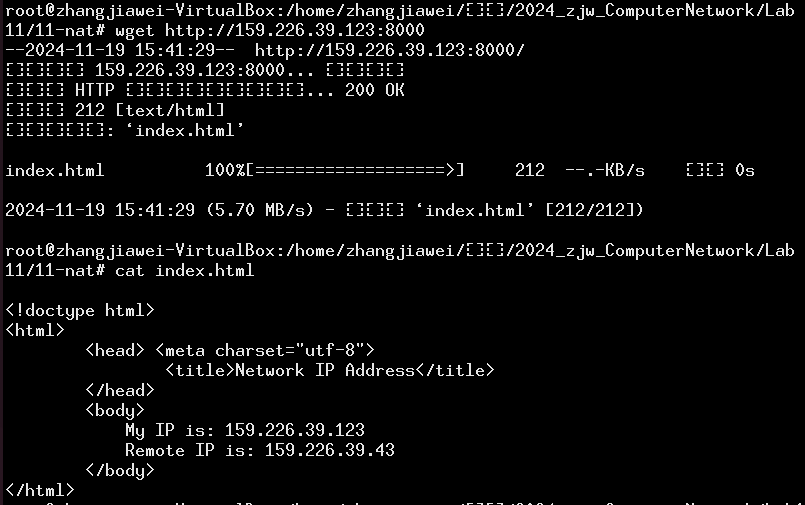
\includegraphics[width=0.8\textwidth]{snat_html_h2.png}
    \caption{h2获取h3页面}
\end{figure}

使用wireshark抓包,结果如下:

\begin{figure}[H]
    \centering
    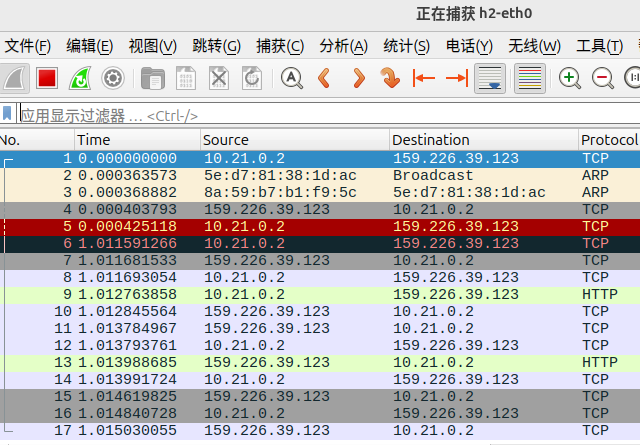
\includegraphics[width=0.8\textwidth]{snat_ws_h2.png}
    \caption{h2获取h3页面抓包h2结果}
\end{figure}

\begin{figure}[H]
    \centering
    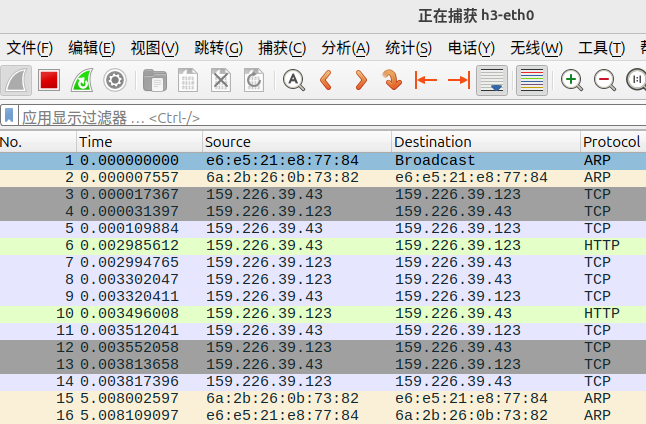
\includegraphics[width=0.8\textwidth]{snat_ws_h3.png}
    \caption{h2获取h3页面抓包h3结果}
\end{figure}

可见,h2成功获取到了h3的页面,且NAT成功将私有地址转换为公有地址。

\subsection{DNAT}

在n1上运行nat程序,读入配置文件exp2.conf,配置文件如下:

\begin{lstlisting}
    internal-iface: n1-eth0
    external-iface: n1-eth1
    
    dnat-rules: 159.226.39.43:8000 -> 10.21.0.1:8000
    dnat-rules: 159.226.39.43:8001 -> 10.21.0.2:8000
\end{lstlisting}

在h3上进行wget操作,结果如下:

\begin{figure}[H]
    \centering
    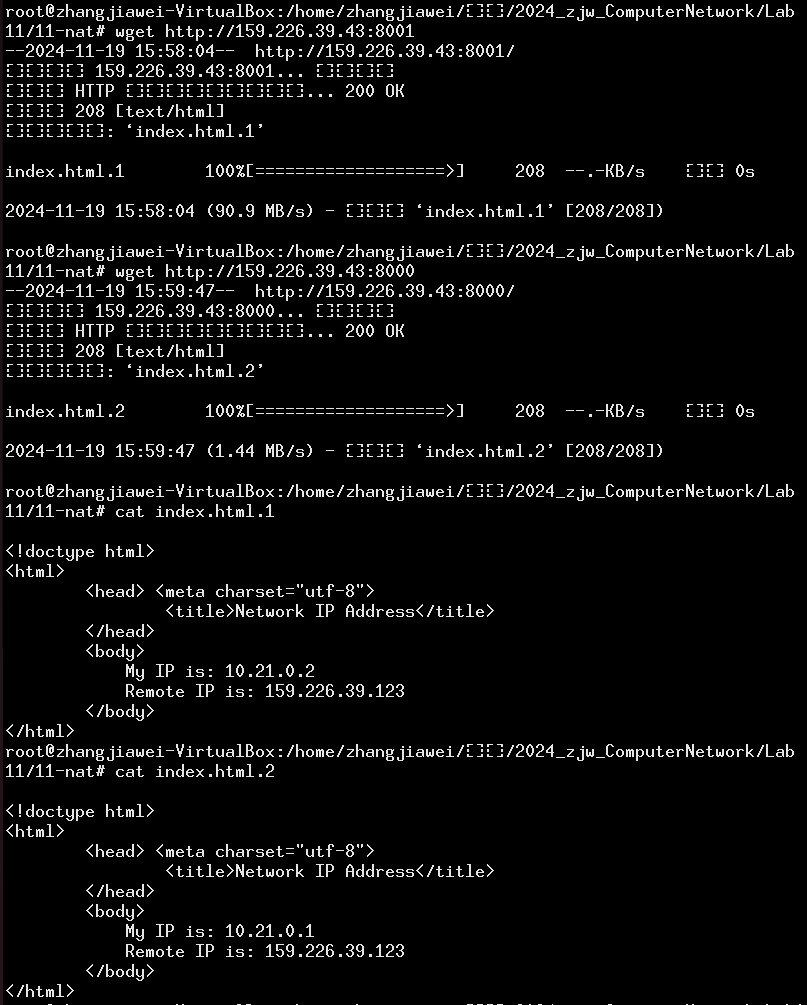
\includegraphics[width=0.8\textwidth]{dnat_html_h3.png}
    \caption{h3获取h1, h2页面}
\end{figure}

使用wireshark抓包,结果如下:

\begin{figure}[H]
    \centering
    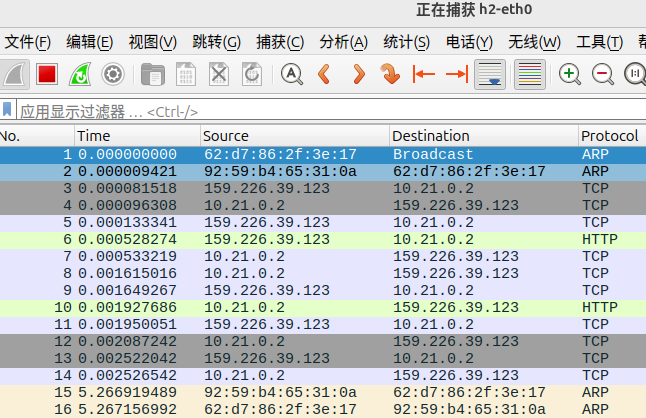
\includegraphics[width=0.8\textwidth]{dnat_ws_h2.png}
    \caption{h3获取h2页面抓包h2结果}
\end{figure}

\begin{figure}[H]
    \centering
    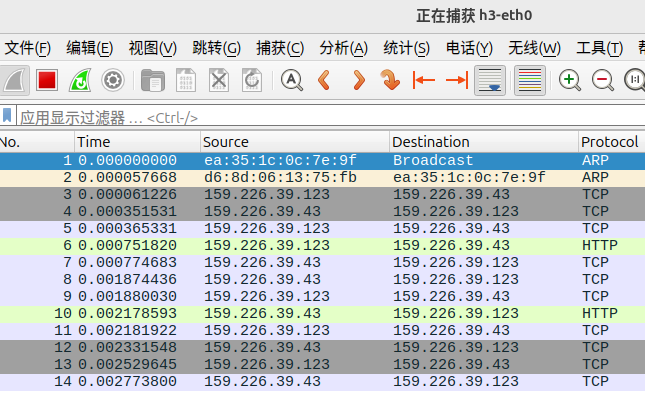
\includegraphics[width=0.8\textwidth]{dnat_ws_h3.png}
    \caption{h3获取h2页面抓包h3结果}
\end{figure}

可见,h3成功获取到了h1和h2的页面,且NAT成功将公有地址转换为私有地址。

\subsection{SDNAT}

手动构造一个包含两个nat的拓扑如下:

\begin{lstlisting}[language=Python]
    h1, h2, n1, n2 = net.get('h1', 'h2', 'n1', 'n2')

    h1.cmd('ifconfig h1-eth0 10.21.0.1/16')
    h1.cmd('route add default gw 10.21.0.254')

    h2.cmd('ifconfig h2-eth0 10.21.0.2/16')
    h2.cmd('route add default gw 10.21.0.254')

    n1.cmd('ifconfig n1-eth0 10.21.0.254/16')
    n1.cmd('ifconfig n1-eth1 159.226.39.23/24')

    n2.cmd('ifconfig n2-eth0 10.21.0.254/16')
    n2.cmd('ifconfig n2-eth1 159.226.39.43/24')
\end{lstlisting}

编写配置文件,分别在n1和n2上运行nat程序并读入配置文件:

\begin{lstlisting}
    internal-iface: n1-eth0
    external-iface: n1-eth1
    
    dnat-rules: 159.226.39.23:8002 -> 10.21.0.1:8000
\end{lstlisting}

\begin{lstlisting}
    internal-iface: n2-eth0
    external-iface: n2-eth1
    
    dnat-rules: 159.226.39.43:8001 -> 10.21.0.2:8000
\end{lstlisting}

令h2提供http服务,在h1上进行wget操作,结果如下:

\begin{figure}[H]
    \centering
    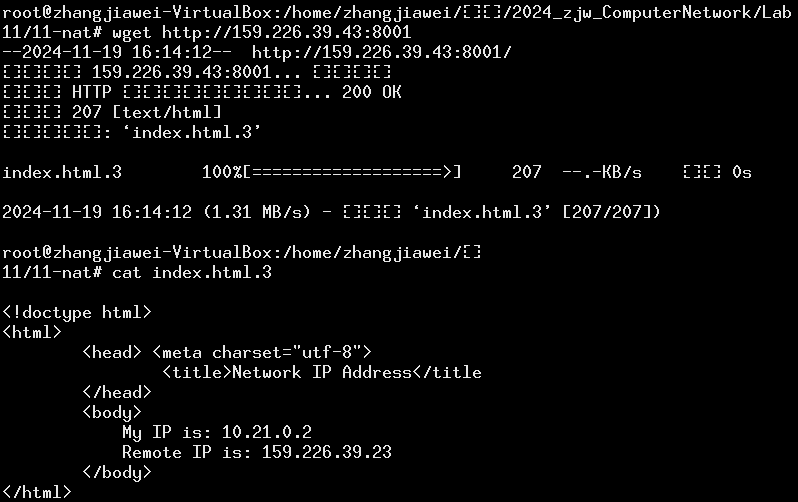
\includegraphics[width=0.8\textwidth]{sdnat_html_h1.png}
    \caption{h1获取h2页面}
\end{figure}

可见,h1成功获取到了h2的页面,且NAT转换成功。

\section{实验总结}

本次实验主要学习了NAT的实现原理,通过实验了解了SNAT、DNAT和SDNAT的实现方法,掌握了NAT的实现过程,与理论知识相结合,加深了对NAT的理解。
\end{document}